\section{Arc Length and The Golden Gate Bridge Problem}
\label{sec:golden_gate_bridge_problem}	

\subsection*{Recommended Tutorials:}
\begin{itemize}[noitemsep]
    \item \nameref{chp:plotting_functions}, pg. \pageref{chp:plotting_functions}
    \item \nameref{chp:equation_solvers}, pg. \pageref{chp:equation_solvers}
	\item \nameref{chp:definite_and_indefinite_Integrals}, pg. \pageref{chp:definite_and_indefinite_Integrals}
\end{itemize}

\subsection*{Introduction:}
Arc length\index{arc length} is the distance between two points along a section of a curve. If this curve can be represented by a function $f(x)$, then we can calculate the length of this curve from $x=a$ to $x=b$ with the formula
\begin{equation}
    \label{eq:arclength}
    L = \displaystyle\int_{a}^b \sqrt{1 + [f^{\prime}(x)]^2}\, dx.
\end{equation}

In this activity, we will determine the arc length of a variety of functions and curves. We can then apply equation \eqref{eq:arclength} above to determine the length of the cable that holds up the Golden Gate Bridge.

\marginnote[-2cm]{You will have to use the \texttt{sqrt()} command to enter this into Maple.}\index{mathematical functions!square root}

\subsection*{Exercises:}

\begin{enumerate}
    \item Consider the function $y = \cos(\sin(x))$.
    \begin{enumerate}
        \item Plot the graph of the function.
        \item Determine the arc length of this curve between the points $(0,1)$ and $(\pi,1)$.\index{Pi}
    \end{enumerate}
    \marginnote[-0.7cm]{Remember that you must type \texttt{Pi} in Maple for $\pi$.}
    \item Consider the curve $y^2 = x^3$.
    \begin{enumerate}
        \item Plot the graph of the curve using \texttt{implicitplot()}.
            \index{packages!plots}
        \item Solve the equation of the curve for $y$ to get the equations of the top and bottom halves of the curves as functions.
        \item Determine the arc length of this curve between the points $(1,1)$ and $(4,8)$.
    \end{enumerate}
    \item Consider the function $x = \frac{1}{3}\sqrt{y}\,(y-3)$.\marginnote[0.1cm]{Don't forget to include multiplication between $\sqrt{y}$ and $(y-3)$.}
   
    \begin{enumerate} \marginnote[0.2cm]{In this exercise, since $x$ is a function of $y$, equation \eqref{eq:arclength} should be an integral in terms of $y$.}
        \item Plot the graph of the function. Since $x$ is defined as a function of $y$, try plotting the equation of the curve using \texttt{implicitplot()}.
        \item Determine the arc length of this curve for $1 \leq y \leq 9$.
    \end{enumerate}
    \item The main span of the Golden Gate Bridge is $1280$ m long, as shown in Figure \ref{fig:goldengate}. The top of each of the towers is 230 m above the surface of the water. To find the length of the cables between these two towers, we will assume that a freely hanging cable between two towers takes the form of a \textbf{catenary}. 
    \marginnote[-2cm]{A catenary is a curve that an idealized hanging chain or cable assumes under its own weight when supported only at its ends. The Golden Gate Bridge cable is almost a catenary and almost a parabola, but not quite either (because of the weight of the cables, the suspender ropes, and the roadway).}
    \clearpage
    \marginnote[0.5cm]{Functions like $\cosh()$ and $\sinh()$ are called hyperbolic functions. These functions are analogs of the ordinary trigonometric, or circular, functions; just as the points $(\cos(t), \sin(t))$ form a circle with a unit radius, the points $(\cosh(t), \sinh(t))$ form the right half of the equilateral hyperbola.}
        \index{mathematical functions!hyperbolic functions!sinh}
         \index{mathematical functions!hyperbolic functions!cosh}
    The general form for a catenary passing through its lowest point at $(0,k)$ is 
    \begin{equation}
        \label{eq:catenary}
        f(x) = a\left(\cosh\left(\tfrac{x}{a}\right)-1\right)+k,
    \end{equation}
    or equivalently,
    \[f(x) = a\left(\frac{{\rm e}^{x/a} + {\rm e}^{-x/a}}{2}-1\right)+k.\]
	
	\begin{figure*}[h]
        \label{fig:goldengate}
        \centering
    	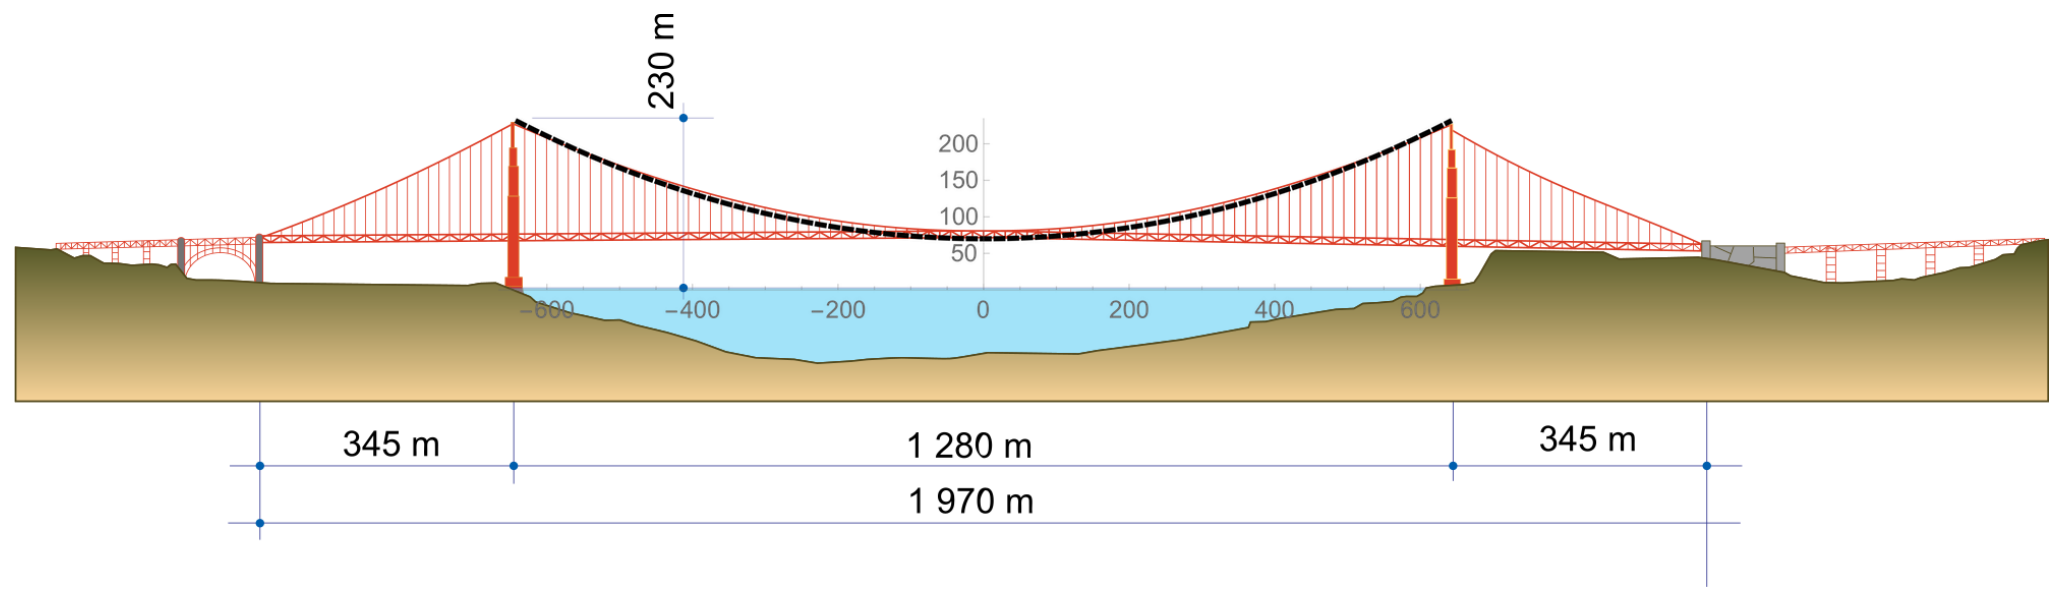
\includegraphics[width=1\linewidth]{activities/math122/figures/goldengate.png}
    	\caption{The portion of the cable for the main span (in black) is approximately the shape of a catenary. The total length of each cable is actually $2{,}332$ m, including the main span and the lengths from both shores.}
    \end{figure*}
    
    Assume that the Golden Gate Bridge cable takes the shape of a catenary over the main span with its lowest point at $(0,70)$, corresponding to a height of $70$ m above the water.
    \begin{enumerate}
        \item Using equation \eqref{eq:catenary} and the points provided in Figure \ref{fig:goldengatesimple}, what is the value of $k$?
        \item Substitute the value of $k$ into \eqref{eq:catenary} and assign this function in Maple.
        \item Use the coordinates of the top of one of the towers from Figure \ref{fig:goldengatesimple}, as well as the \texttt{fsolve()} command to determine the value of $a$ for this catenary.
            \index{solving equations!fsolve}
        \item Using equation \eqref{eq:catenary} with the values of $a$ and $k$ that you have found, determine the length of one of the cables for the main span.
    \end{enumerate}
    
    \begin{marginfigure}[-4cm]
        \hspace{-4cm}
        \centering
        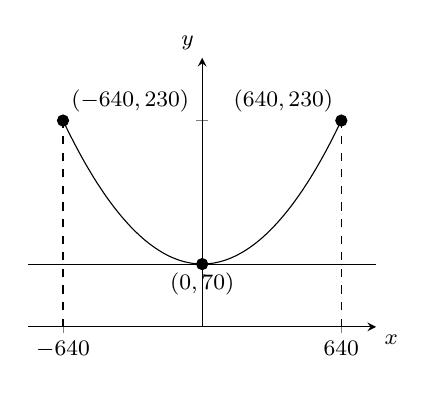
\begin{tikzpicture}
        \footnotesize
        \begin{axis}[
        	width=6cm,
        	height=5cm,
        	axis lines=middle,
        	xlabel={$x$},
        	ylabel={$y$},
        	xlabel style={below right},
        	ylabel style={above left},
        	xmin=-800, xmax=800, xtick={-640,0,640},
        	ymin=0, ymax=300, ytick={0,70,230}, yticklabels={}
        ]
        	\addplot [domain=-640:640, samples=100] {1305.828246*cosh(0.0007657974952*x) - 1235.828246}; %catenary
        	\addplot [domain=-800:800, samples=100] {70}; %bridge deck
        	\addplot[mark=*] coordinates {(-640,230)}; %left tower point
        	\draw(axis cs:-640,230) node [above right] {$(-640,230)$};
        	\addplot[mark=*] coordinates {(640,230)}; %right tower point
        	\draw(axis cs:640,230) node [above left] {$(640,230)$};
        	\addplot[mark=*] coordinates {(0,70)}; %lowest point
        	\draw(axis cs:0,70) node [below] {$(0,70)$};
        	\draw [dashed] (axis cs:-640,0) -- (axis cs:-640,230); %left tower
        	\draw [dashed] (axis cs:640,0) -- (axis cs:640,230); %right tower
        \end{axis}
        \end{tikzpicture}
        \caption{A simplified model of the main bridge span.}
        \label{fig:goldengatesimple}
    \end{marginfigure}
    
    \marginnote[1.5cm]{Interesting fact: The main cables of the Golden Gate Bridge are nearly one meter in diameter (actually, $0.91$ m) and the total length of galvanized steel wire used in both main cables is $129{,}000$ km.}
\end{enumerate}
